\chapter{Language server}
\index{language\_server@\texttt{language\_server}}
\label{chap:lang_server}
The purpose of the Language server is to implement the Language Server Protocol (LSP) and the Debug Adapter Protocol (DAP) and to provide access to the parser library by using them. It has to deserialize and serialize LSP and DAP messages, extract parameters of particular methods and then serve the requests by invoking functionality of parser library.

\section{Language Server Protocol}
Language Server Protocol is used to extend code editors with support for additional programming languages. LSP defines 2 communicating entities: a client and a server. The LSP client is editor-specific and wraps interaction with the user. The LSP server is language-specific and provides information about the source code.

The main purpose of the LSP is to allow the language server to provide language-specific response to various user interactions with the code editor. Messages that flow through LSP can be divided into three categories:

\begin{itemize}
	\item \textbf{Parsing results presentation} Messages from the first category allow the language server to send results of source code analysis to the LSP client. The editor is then able to show them to the user. For example, when the user clicks on a symbol in HLASM code and then uses the `Go to definition' function, the LSP client sends a request to the language server with the name of currently open file and current location in the file. The server is then expected to send back the location of the definition, so the editor can present it to the user (e.g. the editor moves the caret to the definition location). List of all such messages is in \cref{lsp_parse_results}.

	\item \textbf{Editor state and file content synchronization} Messages from the second category flow mainly from the client to the server and ensure that the server has enough information to correctly analyze source code. List of all such messages can be found in \cref{lsp_text_sync_methods}.
	
	\item \textbf{LSP initialization and finalization} Lastly, there are several messages that handle protocol initialization and finalization.
\end{itemize}


\begin{table}
	\centering
	\begin{tabular}{ll}
		
		\toprule
		Message & Description \\ \midrule
		& \multirow{3}{9cm}{The client sends a position in an open file. The server responds with a position of a definition of a symbol at that position.} \\
		textDocument/definition &  \\
		& \\
		& \\
		& \multirow{3}{9cm}{The client sends a position in an open file. If there is a symbol, the server responds with a list of positions where the symbol is used.}\\
		textDocument/references & \\
		& \\
		& \\
		& \multirow{3}{9cm}{The client sends a position in an open file where the user is pointing with the cursor. The server responds with a string to be shown in a tooltip window.}\\
		textDocument/hover & \\
		& \\
		& \\
		& \multirow{3}{9cm}{The client sends a position in an open file and how a completion box was triggered (i.e. with what key, automatically/manually). The server responds with a list of strings suggested for completion at the position.}\\
		textDocument/completion & \\
		& \\
		& \\
		& \\
		\multirow{3}{4cm}{textDocument/\\publishDiagnostics} & \multirow{3}{9cm}{The server sends diagnostics to the client. A diagnostic represents a problem with the source code, e.g. compilation errors and warnings.}\\
		 & \\
		& \\ \bottomrule
	\end{tabular}
	
	\caption{List of all results-presenting messages}
	\label{lsp_parse_results}
\end{table}

\begin{table}
	\centering
	\begin{tabular}{ll}
		
		\toprule
		Message & Description \\ \midrule
		textDocument/didOpen & \multirow{3}{8.5cm}{The server is notified whenever the user opens a file, changes contents of an already open file or closes a file in the editor.} \\
		textDocument/didChange & \\
		textDocument/didClose & \\
		& \\
		 &\multirow{4}{8.5cm}{The client notifies the server when a watched file is changed outside of the editor. Watched files selector is defined when the client is started (in the extension component).} \\
		workspace/ & \\
		didChangeWatchedFiles& \\
		& \\
		& \\
		workspace/ & \multirow{2}{8.5cm}{The client notifies the server that the user has opened or closed a workspace.} \\
		didChangeWorkspaceFolders & \\ \bottomrule
	\end{tabular}
	
	\caption{List of all implemented editor state and text synchronization messages}
	\label{lsp_text_sync_methods}
\end{table}


LSP is based on JSON RPC\footnote{\url{https://www.jsonrpc.org/specification}}. There are two types of interaction in JSON RPC: requests and notifications. Both of them carry the information to invoke a method on the recipient side ---  name of the method and its arguments. The difference between the two is that each request requires a response containing the result of the method, whereas the notifications do not.

The LSP uses the JSON RPC specification and further specifies how messages are transferred and defines methods, their arguments, responses and semantics. A raw message sent from the client to the server is shown in \cref{hover_message}.

\begin{listing}
	\begin{verbatim}
Content-Length: 123\r\n
\r\n
{"jsonrpc":"2.0","method":"textDocument/didClose","params":{"textDocument":
{"uri":"file:/c%3A/Users/admin/Documents/source.hlasm"}}}
	\end{verbatim}
	\caption{An example of a message sent from the client to the server.}
	\label{hover_message}
\end{listing}

The raw messages have HTTP-like headers. The only mandatory header is \TT{Content-Length}, which tells the recipient the length of the following message. The JSON itself is sent after the header.

Inside the JSON, there is a name of the method to be invoked and parameters to pass to the method. In this case, the client is sending a notification that file \TT{C:/Users/admin/Documents/source.hlasm} was closed in the editor by the user. As it is a notification, there must not be any response.

On top of this basic protocol, LSP defines methods and their semantics to cover common functionality that users expect when programming in an editor. List of all methods implemented in the language server can be found in \cref{LSP_methods}.

\section{DAP}
Debug Adapter Protocol is used to extend code editors with debugging support for additional programming languages. We use it to provide the user with the ability to trace how the HLASM compiler processes source code step by step. The user can see the values of compile-time variables and follow the expansion of macros in debug-like experience.

The communication in DAP is between an editor or an IDE and a debugger. The editor notifies the debugger about the user actions, e.g. when a breakpoint is set or when the user uses step in/step over buttons. The debugger informs the editor about the state of the debugged application, for example when the debugger stopped because it hit a breakpoint. While it is stopped, the debugger sends information about program stack, variables valid in current debugger scope and its values.

DAP is very similar to LSP. Although the ideas behind DAP are nearly the same, DAP is not based on the JSON RPC. Instead, DAP specifies its own implementation of remote procedure call, still using JSON as the basic carrier of the messages. DAP has requests and events --- requests always go from the client to the server and require response. Events are the same as the notifications from JSON RPC that are sent from the server to the client. The similarity allows our language server component to share a lot of code between the implementations of the protocols.

\section{Language server overview}
The architecture of the Language server component is illustrated in \cref{lang_server_arch}. It communicates on the standard input/output via LSP with the LSP client and listens on a TCP port to provide DAP support for the macro tracer. The TCP communication is wrapped by class \TT{tcp\_handler}, which abstracts from the complexity of communicating through TCP/IP.


\begin{figure}
	\centering
	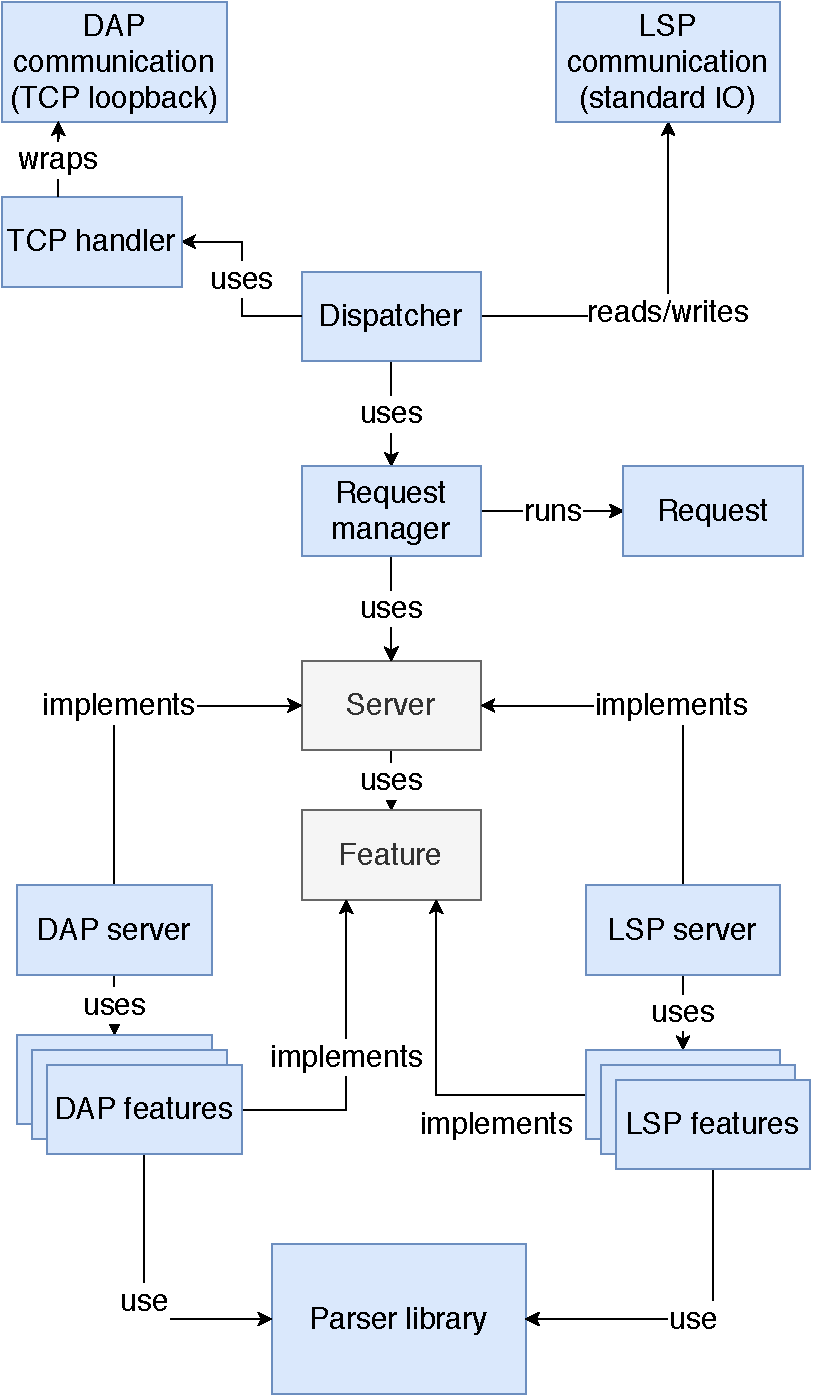
\includegraphics[width=11cm]{img/lang_server}
	\caption{Architecture of language server.}
	\label{lang_server_arch}
\end{figure}


The main purpose of the class \TT{dispatcher} is to provide abstraction for the lowest level communication, which is shared by LSP and DAP. It reads iostream to parse messages using the JSON for Modern C++ library (see \cref{3rd_party}) and stores them in the \TT{request\_manager} as \TT{requests}.

A \TT{request} encapsulates one message that came from the client and is basically represented only by raw (but parsed) JSON.

\TT{request\_manager} stores \TT{requests} in a queue and runs a worker thread that serves the requests one by one. As there is only one instance of request manager running in the language server, it serializes requests from DAP and LSP (which come asynchronously from separate sources) into one queue.

\TT{server} is an abstract class that implements protocol behavior that is common for both DAP and LSP --- it basically implements Remote Procedure Call. Actual handling of LSP and DAP requests is implemented in \TT{features}. Each \TT{feature} contains implementation of several protocol requests or notifications. The features unwrap the arguments from JSON and call corresponding parser library methods.

There are two implementations of the abstract \TT{server} class: \TT{lsp\_server} and \TT{dap\_server}. They both implement the initialization and finalization of protocol communication, which is a bit different for both protocols and both use features to serve protocol requests.

\section{Example: hover request handling}

\afterpage{
	\begin{landscape}
		\begin{figure}
			\centering
			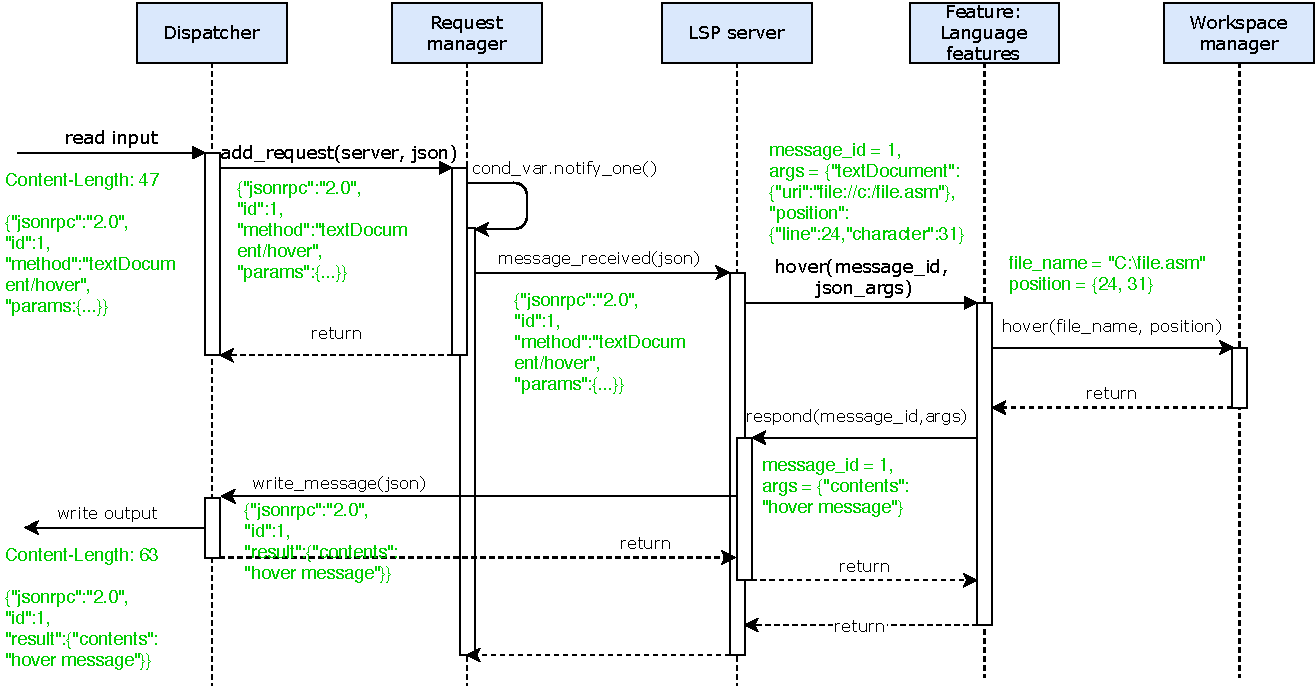
\includegraphics[width=21cm]{img/hover_sequence}
			\caption{A sequence diagram showing the processing of the textDocument/hover request in the language server. The green text represents an example of data passed in the arguments.}
			\label{hover_sequence}
		\end{figure}
	\end{landscape}
}

The \cref{hover_sequence} shows handling of the hover request in the language server. The hover request is sent from the LSP client to the \TT{lsp\_server} when the user hovers over the text of a file. The hover request contains location of the mouse cursor in text, i.e. the name of the file, the number of line and column where the cursor is. The LSP client then expects a response containing a string (possibly written in markdown language) to be shown in a tooltip box.

The whole process begins with reading from the standard input by the LSP instance of the \TT{dispatcher}. It first reads the header of the message, which contains the information about the length of the following JSON. Then it reads the JSON itself and deserializes it using the JSON for Modern C++ library (see \cref{3rd_party}). All other components of the language server work only with the parsed representation of the message. The \TT{dispatcher} adds the message to the \TT{request\_manager} and returns to reading the next message from the standard input.

The request in the \TT{request\_manager} either waits in a queue to be processed, or, if the queue was empty, the worker thread is woken up from sleep using conditional variable. The worker then passes the JSON to the \TT{lsp\_server}, which looks at the name of the method written in the message and calls the method ``hover'' from the language feature.

The hover method unpacks the actual arguments from JSON and converts any URIs to paths using the cpp-netlib URI library. Then, it calls the hover method from the parser library, which returns a string to be shown in the tooltip next to the hovering mouse. The language feature then wraps the return value back in JSON and calls the \TT{respond} method of its \TT{response\_provider} implemented by the \TT{lsp\_server}.

The \TT{lsp\_server} wraps JSON arguments into a LSP response and uses the \TT{send message provider} implemented by \TT{dispatcher} to send it to the LSP client. The \TT{dispatcher} serializes the JSON, adds the header with the length of the JSON and writes the message to a standard output. Finally, all methods return and the worker thread in request manager looks for another request. If there is none, it goes to sleep.

%******************** IO HANDLING *************************
\sectionSrc{I/O handling}
{language\_server/src/main.cpp,language\_server/src/dispatcher.h,language\_server/src/dap/tcp\_handler.h}

The purpose of the \TT{dispatcher} is to abstract from the complexity of working with raw strings and streams. It executes an infinite loop in which it reads messages from \TT{std::iostream} and adds them to the request manager as parsed JSON objects. At the same time, it is able to write responses in the correct format.

The language server communicates with the LSP client on a standard input and output, so we simply use the \TT{dispatcher} with the standard \TT{std::cin} and \TT{std::cout} objects to communicate with the LSP client.

The DAP communicates using TCP/IP, which is less straightforward. Before the VS Code extension starts the language server, it finds a free TCP port and passes it as an argument to the language server executable. The \TT{TCP handler} then starts listening on that port. Once the user wants to start the macro tracer, the DAP client connects to the port on localhost. The \TT{tcp\_handler} accepts the TCP client and creates a \TT{dispatcher} and a \TT{dap\_server}. Once the DAP communication ends, both the \TT{dispatcher} and the \TT{dap\_server} are destroyed and the \TT{tcp\_handler} starts listening again for the next DAP session. Thanks to the ASIO library (see \cref{3rd_party}) implementation of the \TT{std::iostream} interface, the \TT{dispatcher} is able to completely abstract from the fact that it is communicating through TCP and not through the standard IO.

%******************** SERVERS *************************
\sectionSrc{LSP and DAP Server}
{language\_server/src/server.h,language\_server/src/feature.h,language\_server/src/lsp/lsp\_server.h,language\_server/src/dap/dap\_server.h,language\_server/src/dap/dap\_feature.h}
The servers are able to process incoming LSP and DAP requests. They get the messages in a form of already parsed JSONs. Then they extract the name of the requested method with its parameters from the message and call the corresponding method with the parameters encoded as JSON.

There are two server implementations: \TT{lsp\_server} and \TT{dap\_server}. Both inherit from an abstract class called \TT{server}. They implement protocol-specific processing of messages --- although the protocols are quite similar (both are based on RPC), each protocol has different initialization and finalization, different message format, etc.

The functionality of servers is divided into \TT{features}. Each feature implements several LSP or DAP methods by unpacking the arguments of the respective method and calling corresponding parser library function. During initialization, each feature adds its methods to the server's list of implemented methods. The \TT{lsp\_server} uses three features:
\begin{itemize}
	\item \emph{Text synchronization feature}, which handles the notifications about the state of open files in the editor.
	\item \emph{Workspace folders feature}, which handles the notifications about adding and removing workspaces.
	\item \emph{Language feature}, which handles requests about HLASM code information.
\end{itemize}
The \cref{LSP_methods} shows the list of all implemented LSP methods and the classes where the implementations lie.

\begin{table}
	\centering
	\begin{tabular}{lll}
		\toprule
		             \textbf{Component}   &       \textbf{LSP Method name}                                                                                          \\ \midrule
		\multirow{4}{7cm}{LSP server  \\ \srcstyle{language\_server/src/lsp/lsp\_server.h}}                                  & initialize                           \\
		                                                                                                                     & shutdown                             \\
		                                                                                                                     & exit                                 \\
		                                                                                                                     & textDocument/publishDiagnostics      \\ \midrule
		\multirow{4}{7cm}{Text synchronization feature \srcstyle{language\_server/src/lsp/feature\_text\_synchronization.h}} & textDocument/didOpen                 \\
		                                                                                                                     & textDocument/didChange               \\
		                                                                                                                     & textDocument/didClose                \\
		                                                                                                                     & textDocument/semanticHighlighting    \\ \midrule
		\multirow{2}{7cm}{Workspace folders feature \srcstyle{language\_server/src/lsp/feature\_workspace\_folders.h}}       & workspace/didChangeWorkspaceFolders  \\
		                                                                                                                     & workspace/didChangeWatchedFiles      \\ \midrule
		\multirow{4}{7cm}{Language feature \srcstyle{language\_server/src/lsp/feature\_language\_features.h}}                & textDocument/definition              \\
		                                                                                                                     & textDocument/references              \\
		                                                                                                                     & textDocument/hover                   \\
		                                                                                                                     & textDocument/completion              \\ \bottomrule& 
	\end{tabular}
	\caption{The list of all implemented LSP methods and the classes where they are implemented}
	\label{LSP_methods}
\end{table}

The DAP server uses only one feature --- the Launch feature, which handles stepping through the code and retrieving information about both variables and stack trace. The table \cref{DAP_methods} shows the list of all implemented DAP methods.

\begin{table}
	\centering
	\begin{tabular}{lll}
		\toprule
		\textbf{Class}                          & \textbf{Source file}                                                      & \textbf{DAP Method name} \\ \midrule
		\multirow{2}{3cm}{\TT{DAP server}}      & \multirow{2}{3cm}{\srcstyle{language\_server/src/dap/dap\_server.h}}      & \TT{initialize}          \\
		                                        &                                                                           & \TT{disconnect}          \\ \midrule
		\multirow{13}{3cm}{\TT{Launch feature}} & \multirow{13}{3cm}{\srcstyle{language\_server/src/dap/feature\_launch.h}} & \TT{launch}              \\
		                                        &                                                                           & \TT{setBreakpoints}      \\
		                                        &                                                                           & \TT{configurationDone}   \\
		                                        &                                                                           & \TT{threads}             \\
		                                        &                                                                           & \TT{stackTrace}          \\
		                                        &                                                                           & \TT{scopes}              \\
		                                        &                                                                           & \TT{next}                \\
		                                        &                                                                           & \TT{stepIn}              \\
		                                        &                                                                           & \TT{variables}           \\
		                                        &                                                                           & \TT{continue}            \\
		                                        &                                                                           & \TT{stopped}             \\
		                                        &                                                                           & \TT{exited}              \\
		                                        &                                                                           & \TT{terminated}          \\ \bottomrule
	\end{tabular}
	\caption{The list of all implemented DAP methods and the classes where they are implemented}
	\label{DAP_methods}
\end{table}

%******************** RESPONSE *************************
\sectionSrc{Response with result}
{language\_server/src/feature.h,language\_server/src/server.h}

According to the LSP and the DAP, the server is required to send messages back to the LSP/DAP client either as responses to requests (e.g. \TT{hover}), notifications (e.g. textDocument/publishDiagnostics notification) or events (e.g. stopped event). Features require reference to an instance of the \TT{response\_provider} interface that provides methods \TT{respond} and \TT{notify} for sending messages back to the LSP client. Both LSP and DAP server classes implement the \TT{response\_provider} to form protocol-specific JSON with the arguments.

The servers then send the JSON to the LSP/DAP client using the \TT{send\_message\_provider} interface. At this point, the final complete JSON response is formed. The \TT{send\_message\_provider} then adds the message header and serializes the JSON using the JSON for Modern C++ library (see \cref{3rd_party}).

The only implementation of the \TT{send\_message\_provider} interface is the \TT{dispatcher}.

%******************** REQUEST MANAGER *************************
\sectionSrc{Request Manager}
{language\_server/src/request\_manager.h}

\TT{Request manager} encapsulates a queue of requests with a worker thread that processes them. There may be up to two \TT{dispatcher} instances in the language server: one for LSP and one for DAP. Both of them add the requests they parse into one \TT{request manager}. It is necessary to process the requests one by one, because the parser library cannot process more requests at the same time.

There are three threads running in the language server:
\begin{itemize}
	\item LSP read thread --- a thread in which the \TT{dispatcher} reads messages from the standard input.
	\item DAP read thread --- a thread in which the \TT{tcp\_handler} listens on a localhost port to initiate a DAP session. After accepting the DAP client, the \TT{dispatcher} reads DAP input on this thread too.
	\item Worker thread in \TT{request\_manager} that processes each request using the \TT{lsp\_server} or the \TT{dap\_server} and ultimately the parser library.
\end{itemize}

The threads are synchronized in two ways: First, there is a mutex that prevents the LSP and the DAP threads from adding to the request queue simultaneously. Second, there is a conditional variable to control the worker thread.

Request manager additionally incorporates a mechanism for invalidating requests that have been obsoleted by new requests. The obsoleting of requests is done by a cancellation token. It is shared between the parser library and the \TT{request\_manager}. When set to true, the results of current request or notification are no longer needed, the parser library stops all parsing and return as soon as possible.

When a new request arrives, all previous requests (including the currently processed one) that concern the same file are invalidated. However, they cannot be simply removed from the queue. They still have to be processed as they may carry information that must not be discarded (e.g. changes to contents of a file). The parser library processes the request but does not reparse any source files.

\subsection{Example of request invalidating}

For example, when a user starts changing a file, every character he writes is passed to the language server as a textDocument/didChange notification. Each such notification is processed in two stages:
\begin{enumerate}
	\item The parser library changes the internal representation of the text document.
	\item The parser library starts the parsing of the file to update diagnostics and highlighting. This may take some time.
\end{enumerate}
When more didChange notifications come in succession, their first parts must be executed with all the notifications to keep the internal representation of the file updated. However, the user is interested only in diagnostics and semantic highlighting for the current state of the text, so we need to parse the file only once --- after the last notification.



